\chapter{Asterisk, an open source PBX}
\section{Overview}
Created in 1999, Asterisk is designed to be an open-source telephony server. Multi-platform, it can be used in lot of various application. It can also easily manage both physical phone devices and phones software. More globally, a PBX is able to create automated vocal services, internal company phone service, voice mails... And it is just some examples of a PBX usage.

\section{Why Asterisk?}
For this project, we tried to look for an efficient telephony server. A server with a lot of documentation and a great community support would be ideal. Moreover, this server should be really flexible because the configuration will be often generated, and then reloaded.
Because lot of these PBX are managed by a web GUI interface, we discovered \textit{Asterisk}. It seemed to be the ideal server we needed. It have an excellent community support, a great documentation and able to reload its configuration fastly without interrupting current communications.

\section{Server compilation}
Because \textit{Asterisk} is provided as open source server, we had to download the server sources and then compile them with the following commands:
\begin{lstlisting}[language=bash,caption={bash}]
$ ./configure
$ make menuconfig
$ make
$ make install
\end{lstlisting}

One of the most important command in the above list was \textit{make menuselect}: this command allows to enable and disable unwanted modules. It is there we can enable for example the MP3 support.

\section{Server organization}

\subsection{Contexts}
On Asterisk, all phone activities are based on contexts. It means when a phone is registered in a context, it can't reach phones which are located in different context. The contexts will be mainly useful for the company switchboard. Indeed, all switchboard will have their own context called like "\textbf{SWITCHBOARD\_USER\_(CODE)}" where (CODE) is replaced by the switchboard access code, defined at the creation of the switchboard on the website.


\textit{ScotIP} purposes two kinds of lines: the dedicated line and the shared lines.
Shared lines will share the same starting context. This context is called \textbf{ScotIPHome}. It is a vocal service where all incoming calls will be redirected. This vocal service will ask the caller to enter the switchboard access code, and if it exists, then the caller will be redirected on the switchboard context.


This is possible thanks to variables, conditions and functions provided in Asterisk. When the caller will press his phone keys, the number will be stored in a temporary variable. Then, thanks to the function \textbf{DIALPLAN\_EXISTS(name)} the caller can be redirected on the right context. Otherwise, the call will be hang up. 

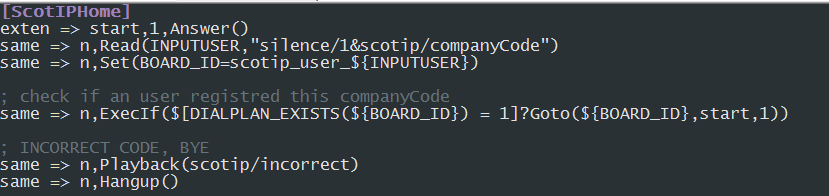
\includegraphics[width=1\textwidth]{img/context_scotiphome.png}


\subsection{Files and \#include directive}

Because Asterisk configuration have to be located in \textit{/etc/asterisk} directory, the configuration can't be flexible. However, one directive exists to bypass this obligation. \textbf{\#include}. Thanks to this directive, we could organize our server architecture in many subdirectories. This directive allows also the use of \textit{jokers}, represented by this character: \textbf{*}. In our application, we chose to save all these files to the directory \textit{/usr/scotip}.

Each directory will match one type of configuration file. For example, we have to save the dialplans for the company switchboards, music on hold files, extensions configuration... 

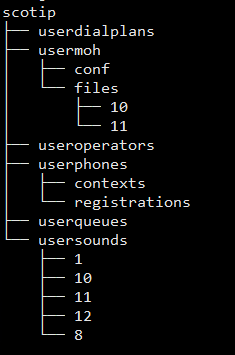
\includegraphics[scale=1]{img/files_struct_conf.png}

\section{SIP}

\subsection{SIP peers}
In order to emit and receive calls, we have to register on the network on our providers. To use these networks, there are two important steps. 


First, we have to write a registration string of this kind: \textit{register => username:password@provider.dot.ltd}. This line allows to register our server to use the provider network. The state of this connection through the command line: \textit{sip show registry}

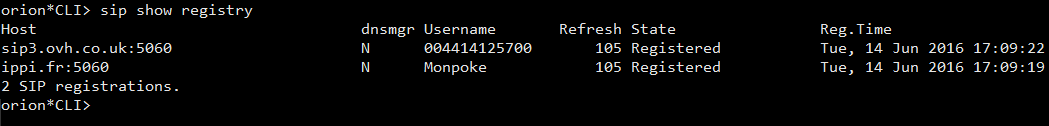
\includegraphics[width=1\textwidth]{img/sipshowregistry.png}


For the second step, we have to tell Asterisk in which context the incoming calls have to be redirected, and also make some settings on the connection. (Eg: monitoring, incoming host...)
Because on our project we only made possible incoming calls, we will not talk about outgoing calls in this report. For all these calls, they will be redirected on a local context called \textbf{phone\_incoming}, then redirected on a global context for all the project: \textbf{ScotIPHome}, which have been previously described.

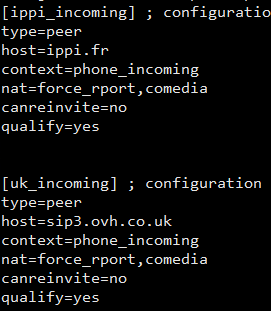
\includegraphics[width=1\textwidth]{img/contextsphones.png}

\subsection{Extensions}


\subsection{Calling Skype account}


\section{Dialplan and applications}

\subsection{Playback}
\subsection{Queue}
\subsection{Operator}
\subsection{Playback}
\subsection{User input}



\section{MOH}
\subsection{About}
\subsection{Conversion}
Not here, but in website 